% Created 2023-10-21 Sat 10:43
% Intended LaTeX compiler: pdflatex
\documentclass[11pt]{article}
\usepackage[utf8]{inputenc}
\usepackage[T1]{fontenc}
\usepackage{graphicx}
\usepackage{longtable}
\usepackage{wrapfig}
\usepackage{rotating}
\usepackage[normalem]{ulem}
\usepackage{amsmath}
\usepackage{amssymb}
\usepackage{capt-of}
\usepackage{hyperref}
\usepackage{placeins}
\usepackage{gensymb}
\author{Christian}
\date{\today}
\title{}
\hypersetup{
 pdfauthor={Christian},
 pdftitle={},
 pdfkeywords={},
 pdfsubject={},
 pdfcreator={Emacs 28.2.50 (Org mode 9.7-pre)}, 
 pdflang={English}}
\begin{document}

\section*{Part A}
\label{sec:orgb6365eb}
\begin{verbatim}
set.seed(1)
data=rbinom(1000000,1,0.9)
dim(data)=c(100000,10)
sumofrows=apply(data,1,sum)
data2=rbinom(100000,10,0.9)
par=(mfrow=c(2,1))
vectorofbreaks=seq(from=-0.5,to=10.5,by=1)
hist(sumofrows,breaks=vectorofbreaks)
hist(data2,breaks=vectorofbreaks)
\end{verbatim}

\begin{figure*}
\centering
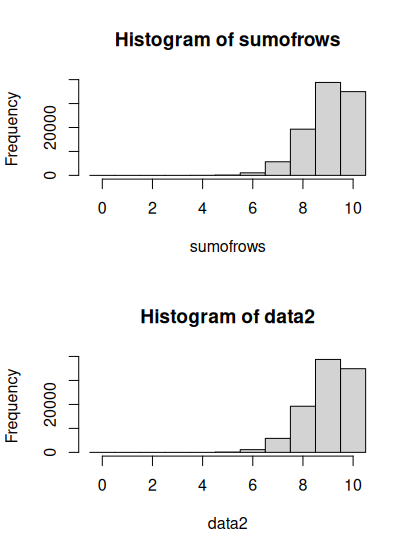
\includegraphics[width=.9\linewidth]{/home/csj7701/class/F23/Prob Theory/Project1/Histograms.png}
\bicaption{---}
\end{figure*}

First 5 rows of \texttt{data}:

\begin{center}
\begin{tabular}{lrrrrrrrrrr}
 & [,1] & [,2] & [,3] & [,4] & [,5] & [,6] & [,7] & [,8] & [,9] & [,10]\\[0pt]
[1,] & 1 & 1 & 1 & 1 & 1 & 1 & 1 & 1 & 1 & 1\\[0pt]
[2,] & 1 & 1 & 1 & 1 & 1 & 1 & 1 & 0 & 1 & 1\\[0pt]
[3,] & 1 & 1 & 1 & 1 & 1 & 1 & 1 & 1 & 1 & 0\\[0pt]
[4,] & 0 & 1 & 1 & 1 & 1 & 1 & 1 & 0 & 1 & 1\\[0pt]
[5,] & 1 & 1 & 1 & 1 & 1 & 1 & 1 & 1 & 1 & 1\\[0pt]
\end{tabular}
\end{center}

First 5 entries of \texttt{sumofrows}

\begin{center}
\begin{tabular}{lrrrrr}
[1] & 10 & 9 & 9 & 8 & 10\\[0pt]
\end{tabular}
\end{center}

First 5 entries in \texttt{data2}

\begin{center}
\begin{tabular}{lrrrrr}
[1] & 10 & 9 & 9 & 10 & 10\\[0pt]
\end{tabular}
\end{center}


Do the Histograms look the same?
\begin{itemize}
\item Yes.
\end{itemize}
Why, and should they?
\begin{itemize}
\item The two histograms look almost identical because of the way we average data to create \texttt{sumofrows}.
\texttt{data} begins as a matrix with 100,000 rows and 10 columns. \texttt{sumofrows} averages each row to find the marginal distribution, resulting in a 100,000 element vector.
When we create \texttt{data2}, we are making a vector of 100,000 elements that follows the same probability of success as \texttt{data}, and by finding the marginal distribution of \texttt{data}, we have ensured that it maintains the same general probability.
This means that \texttt{sumofrows} and \texttt{data2} should be nearly identical from a general perspective.

--> We're essentially "averaging" \texttt{data} so that it will maintain the same slope/shape, but have fewer elements.
\end{itemize}
\section*{Part B}
\label{sec:org36a519d}

Summary(tr)
\begin{center}
\begin{tabular}{lrr}
mode & FALSE & TRUE\\[0pt]
logical & 10027 & 89973\\[0pt]
\end{tabular}
\end{center}

Calcualated probability of first success on first trial:
\(0.9^{1}=0.9\)

Summary(tr2)
\begin{center}
\begin{tabular}{lrr}
mode & FALSE & TRUE\\[0pt]
logical & 90949 & 9051\\[0pt]
\end{tabular}
\end{center}

Calculated probability of first success on second trial:
\(\binom{1}{0}*0.9^{1}*0.1^{1}=0.09\)

Explanation of data summaries:

As explained in the lab document, \texttt{tr} finds every instance of 1 in the first column, registering \texttt{1} as a logical \texttt{true} and \texttt{0} as \texttt{false}. \texttt{tr2} finds every instance of 0 in the first column, then given that, every instance of \texttt{1} in the second column where the first column is 0.

This gives us likelihood of the first success on first trial (\texttt{tr}) and likelihood of first success on second trial (\texttt{tr2}).
When we calculate the mathematical probability of sucess on first trial, we get \(0.9\), which is similar to what we got from our R code (Since \(\frac{89973}{89973+10027}=0.8997\)).

Similarly, when we calculate the mathematical likelihood of first success on second trial, we get \(0.09\), which is also similar to what we got from our R code (since \(\frac{9051}{9051+90949}=0.09053\))
\end{document}